\section{Discharges and currents}\label{app:discharges}
\sectionstate{ready}{\texttt{rerun/paper1\_ops/README.md} (recovery after a discharge), \texttt{rerun/paper1\_ops/currents/README.md}
(currents); corrections from \texttt{papers/paper1\_v2/NUMBERS\_RUNDOWN.md} items 4, 5, 10, 11 and \texttt{figs/out/gain\_scan.json}.
v2 2026-11-10: the old appendix B and the dark-current paragraph and figures of the old section 4.}
\intent{This appendix answers: what does a discharge cost, and what current do the chambers draw?}

\subsection{Recovery after a discharge}\label{app:recovery}
Three quantities have to be kept apart. The reconstruction sets aside any trigger with more than 50 strips above
threshold. A \emph{discharge} is such a trigger in which at least one readout chip has eight or more strips above
3000 ADC counts. At 490\,V about 4\,\% of the triggers of chamber~A are discharges, and 0.9\,\% of its reference tracks
fall in one; the loss class called discharge in \cref{tab:losses} is the part of those confirmed as a real discharge
by its ringing.

Each reference-matched track is placed by the time since the last discharge on its chamber, and its detection
efficiency and median charge are compared with tracks more than 1\,s after a discharge (\cref{fig:sparkdt}). Neither
moves at any delay we resolve. The efficiency in the first bin, 0--3\,ms after a discharge, is already $1.07\pm0.04$
of its late value (chamber~A, 53 tracks). Integrating the efficiency deficit over the first 0.1\,s after a discharge,
the dead time per discharge is $0.2\pm0.6$\,ms for chamber~A, below 1.2\,ms at 95\,\% confidence; for chambers B, C
and D the limits are 2.1, 2.6 and 2.1\,ms, and for chamber~E, with few discharges, 15.5\,ms. The cosmic rate does not
resolve the recovery itself, so these are bounds and not a measurement of it.
\begin{figure}[tbp]
  \centering
  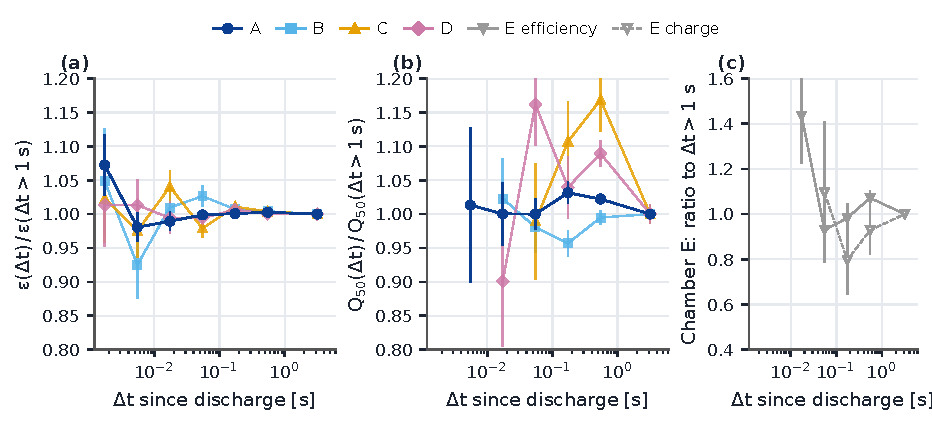
\includegraphics[width=\linewidth]{spark_deadtime}
  \caption{(a) Detection efficiency and (b) median charge against the time since the previous discharge, each
  relative to its value more than 1\,s after it; (c) chamber~E on its own scale. Discharges: A 45\,500, B 17\,208, C
  24\,126, D 42\,827, E 4\,303. Charge errors from a bootstrap. Fitted dead time per discharge: A $0.2\pm0.6$, B
  $-1.7\pm1.3$, C $0.8\pm1.1$, D $0.4\pm1.1$, E $-2.4\pm9.4$\,ms.}
  \label{fig:sparkdt}
\end{figure}

\subsection{Dark current}\label{app:current}
The resistive strips draw a steady current far above the signal current. For chamber~A, alone on the bench on 27
June (\cref{fig:currents}), the current is flat at 0.17--0.18\,\textmu A below 460\,V (0.2--0.3\,\textmu A on other
nights) and above about 465\,V it doubles every $13.3\pm0.3$\,V,
$I=(1.05\pm0.05)\,\text{\textmu A}\times2^{(V-490\,\text{V})/13.3\,\text{V}}$. Between 470 and 495\,V, where both are
measured, the current grows by a factor 5.4 while the track charge grows by 3.0, so the current rises faster than the
gain, as $G^{1.5\pm0.1}$. It does not depend on the drift field (1.03--1.11\,\textmu A for 100 to 1100\,V on the
cathode). At the working point this is about 1\,\textmu A, $10^5$ times the signal current of cosmic rays (about
4\,pA). It is a gain-driven dark current of the amplification stage, of a family with the noise bands that sit on
fixed patches of strips, whose rate goes as $G^{1.4-1.6}$, and with the discharges ($G^{2-2.7}$). Across boards at
490\,V: C 0.45, E 0.58, A 0.29--1.14 (night to night), B 1.0--2.4 and D 6.0--6.4\,\textmu A, the last being the chamber
with the most discharges (\cref{fig:currents_all}). The mechanism is not identified.
\askDylan{Changed from the old text. ``No measurable ohmic part'' is gone: the fitted constant is $0.01\pm0.04$\,\textmu A, but
that fit misses the measured 0.17\,\textmu A foot at 425--455\,V by 0.06--0.12\,\textmu A. ``$I\propto G^{1.25}$'' is gone: it compared
a current slope from 490--525\,V with a gain slope from below 465\,V. ``The same scaling as the noise bands'' is now ``of a
family with'', since the exponents differ.}
\begin{figure}[tbp]
  \centering
  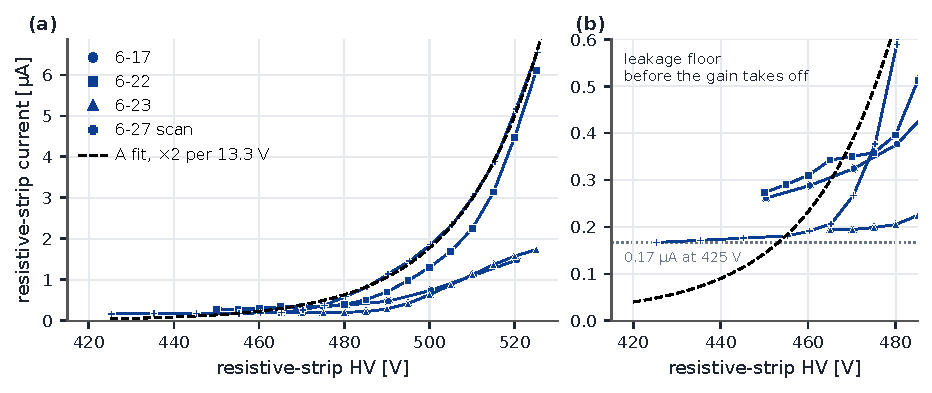
\includegraphics[width=\linewidth]{currents_vs_hv}
  \caption{Current of the resistive strips of chamber~A against $HV_\mathrm{resist}$ on four nights (markers: the
  overnight runs of 17, 22 and 23 June; the scan of 27 June). (a) Full range, linear scale; dashed: the fit to the
  scan, $I=1.05\,\text{\textmu A}\times2^{(V-490\,\text{V})/13.3\,\text{V}}$. (b) The same data below 485\,V: before the
  gain takes off the current is flat at about 0.2\,\textmu A, which the exponential does not follow.}
  \label{fig:currents}
\end{figure}
\begin{figure}[tbp]
  \centering
  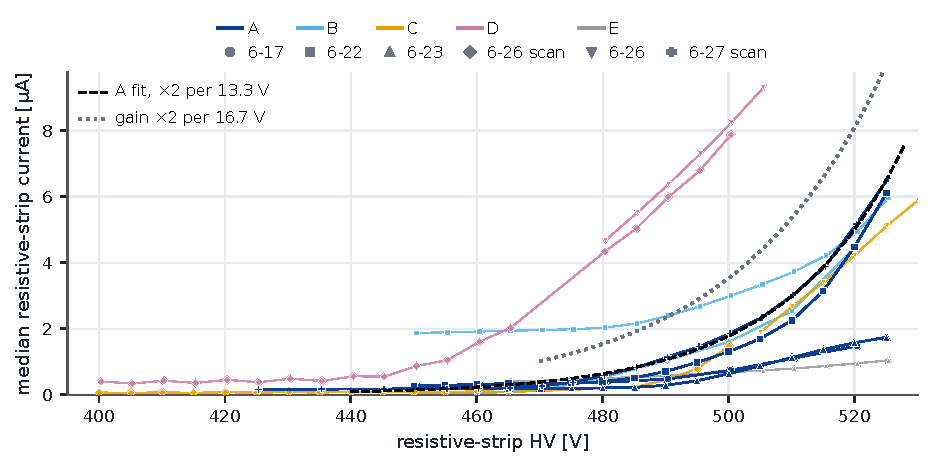
\includegraphics[width=\linewidth]{currents_vs_hv_all}
  \caption{Current of the resistive strips against $HV_\mathrm{resist}$ for every board, from 17 June on. Colour:
  chamber; marker: night (``scan'': days of voltage scans; other dates: overnight runs). Dashed: the fit of
  \cref{fig:currents}. Linear scale.}
  \label{fig:currents_all}
\end{figure}
